\section*{Exercice 148 -- Cinématique}
\setcounter{exo}{0}

On note $\theta=\angl{x}{x_1}$, $\phi=\angl{y_1}{y_2}$, 
$\vect{AB}=R\vect{x_1}$ et $\vect{BP}=L\vect{y_2}$.

\begin{center}
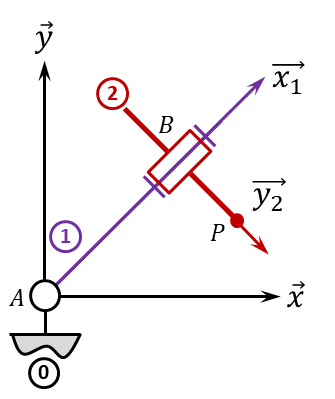
\includegraphics[width=.8\linewidth]{972_01}
\end{center}

\subparagraph{}
\textit{Tracer les figures planes.}
\ifprof
\begin{corrige}

\end{corrige}
\else
\fi

\subparagraph{}
\textit{Déterminer $\vectv{P}{2}{0}$.}
\ifprof
\begin{corrige}

\end{corrige}
\else
\fi

\subparagraph{}
\textit{Déterminer $\vectg{P}{2}{0}$.}
\ifprof
\begin{corrige}

\end{corrige}
\else
\fi
